\section{実験概要}
実ロボットを用いて, 提案するシステムにより, 
ロボットが目的地へ到達可能であるか検証する.
\subsection{実験装置}
実験で用いるロボットを\ref{fig:gamma}に示す.
ロボットはicart-mini\cite{icart}をベースに本研究室で開発した
orne\_gammaを用いる.
センサとして,単眼のウェブカメラ(サンワサプライ株式会社 CMS-V43BK)を3つ,
2D-LiDAR(北陽電機 UTM-30LX)を1つ搭載している. 
また左右のモータにそれぞれパルス付きエンコーダが付属している.
制御用の PC には GALLERIA GCR2070RGF-QC-Gを使用している.
メトリックマップに基づくナビゲーションには,本学でNavigation stackをもとに開発した
orne\_navigation\cite{orne_nav}を使用する
\begin{figure}[htbp]
    \centering
     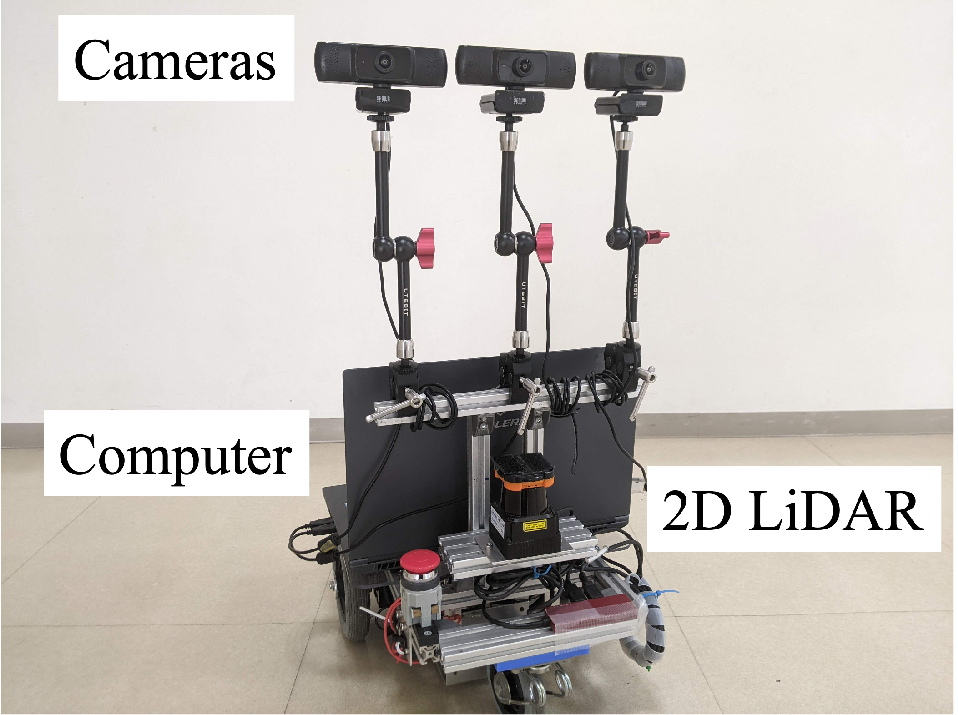
\includegraphics[width=80mm]{images/pdf/gamma_sensor.pdf}
     \caption{Experimental setup}\label{fig:gamma}
\end{figure}

\newpage
\subsection{実験方法}
実験環境として\ref{fig:cit3f}に示す千葉工業大学津田沼キャンパス2号館3階の廊下を用いる.
環境中には,三叉路が4つ,角が2つ,突き当たりが2つ含まれている.
経路追従モジュールの訓練および通路分類モジュールのデータセット収集では,
\ref{fig:newroute}で示したaからnの経路を順番に走行する.
\begin{figure}[htbp]
    \centering
     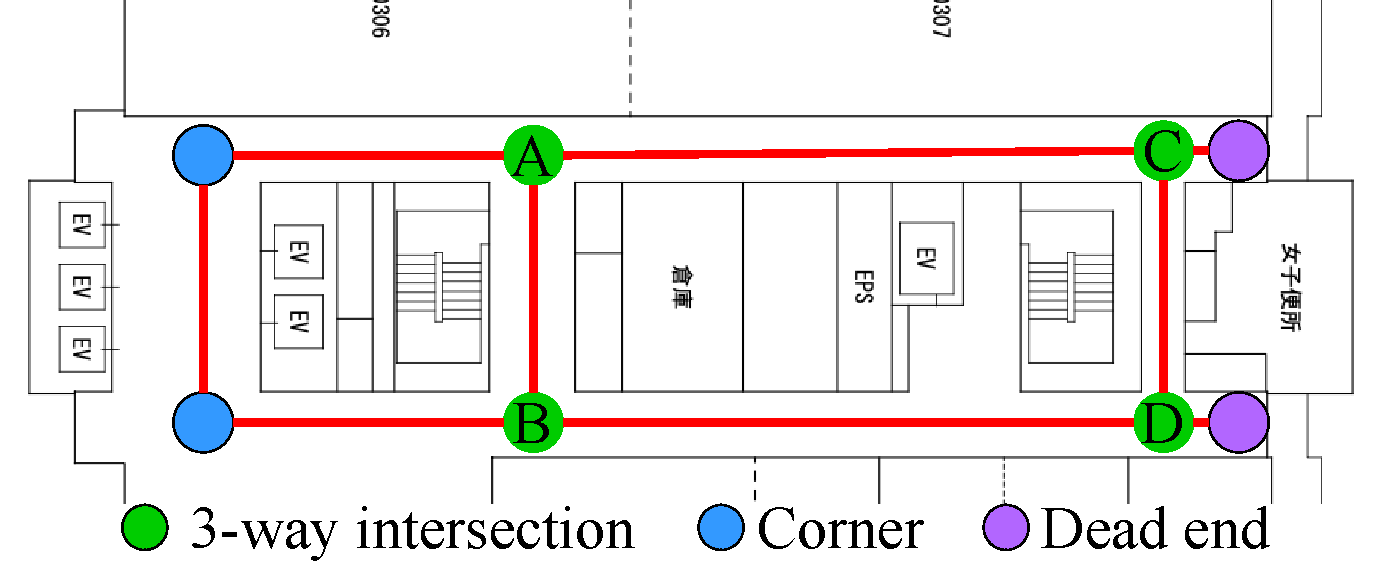
\includegraphics[width=100mm]{images/pdf/cit3f.pdf}
     \caption{Experimental environment \cite{haruyama2023}}\label{fig:cit3f}
\end{figure}
\begin{figure}[htbp]
    \centering
     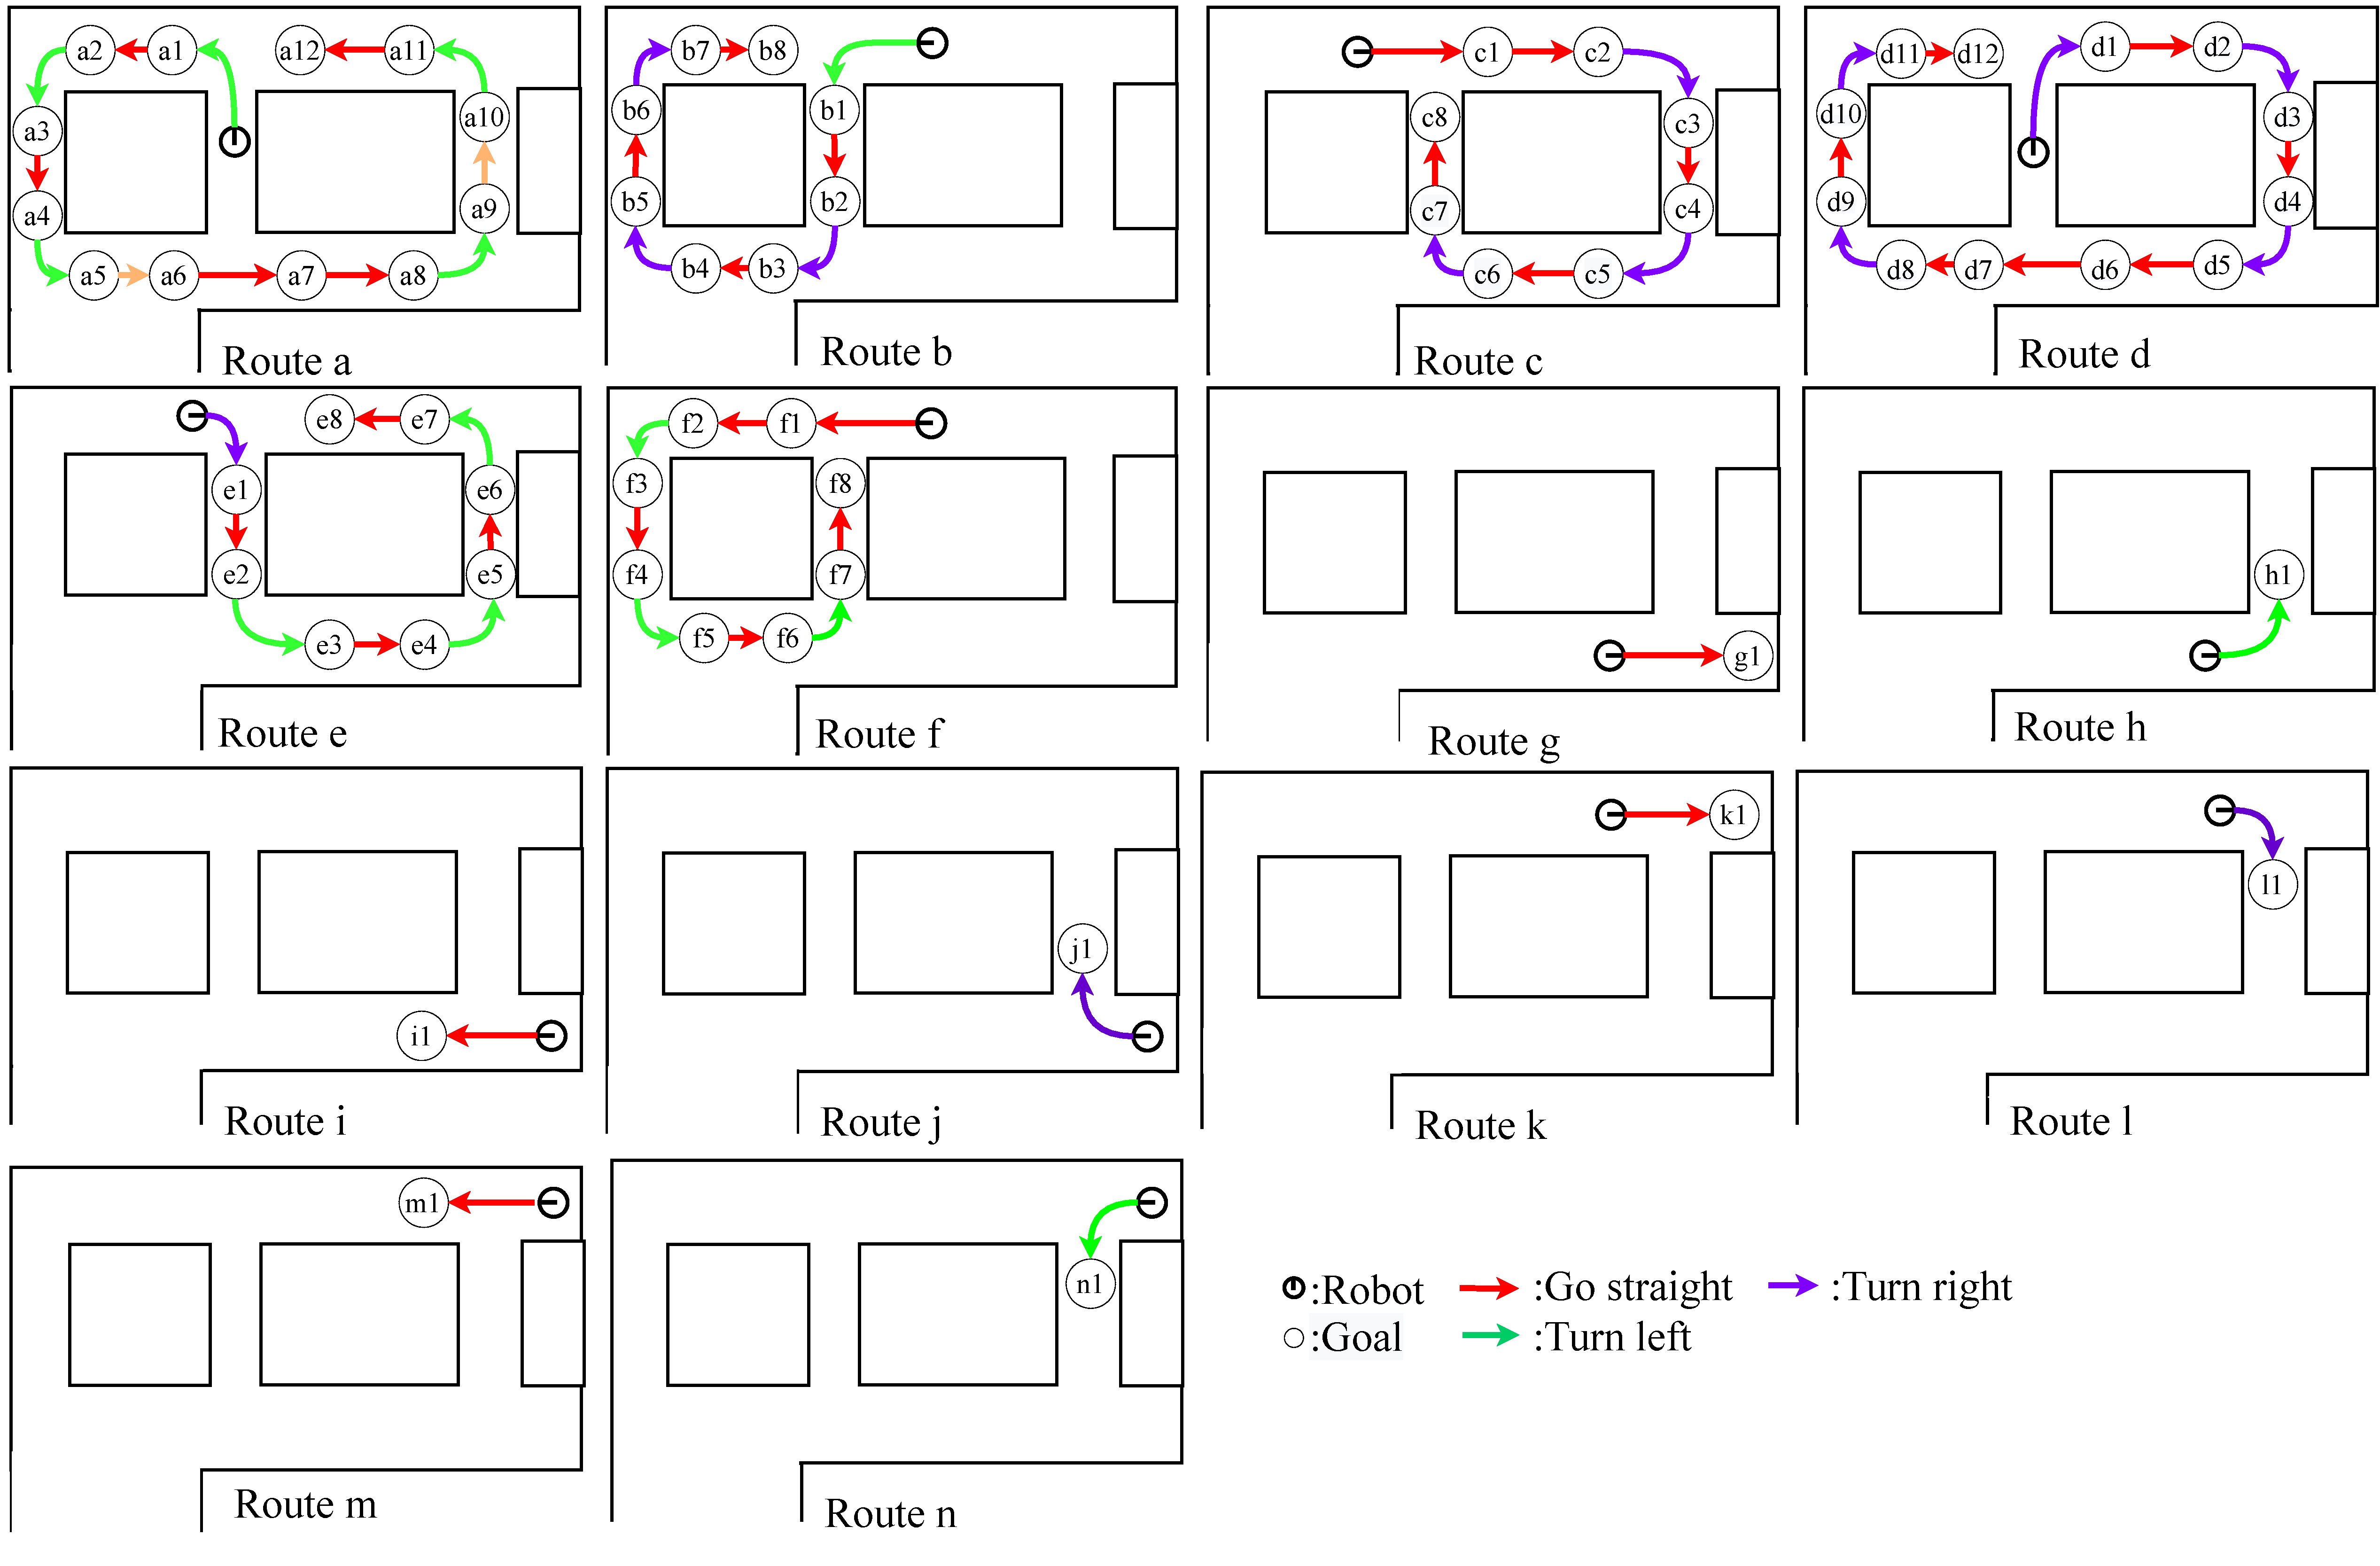
\includegraphics[width=130mm]{images/pdf/newroute.pdf}
     \caption{Experimental environment Quoted from \cite{haruyama2023}}\label{fig:newroute}
\end{figure}


\subsubsection{シナリオの選定}
実験では島田らが用いた50例のシナリオの中から,
〜に示す7例を用いた.
このシナリオは以下の3つの基準に従って,選定した.
% \ref{fig:cit3f}の場所を対象としていること.
% ロボットが移動困難な\ref{fig:semai}の箇所のような狭い通路が含まれていないこと.
% その場で「後ろを向く」など経路追従モジュールができない行動が含まれていないことである.
\begin{enumerate}
    \item [1)] \ref{fig:cit3f}の場所を対象としていること.
    \item [2)] ロボットが移動困難な\ref{fig:semai}の箇所のような狭い通路が含まれていないこと
    \item [3)] その場で「後ろを向く」など経路追従モジュールができない行動が含まれていないこと
\end{enumerate}

\begin{figure*}[htbp]
    \begin{tabular}{ccc}
        \begin{minipage}[t]{0.5\textwidth}
            \centering
            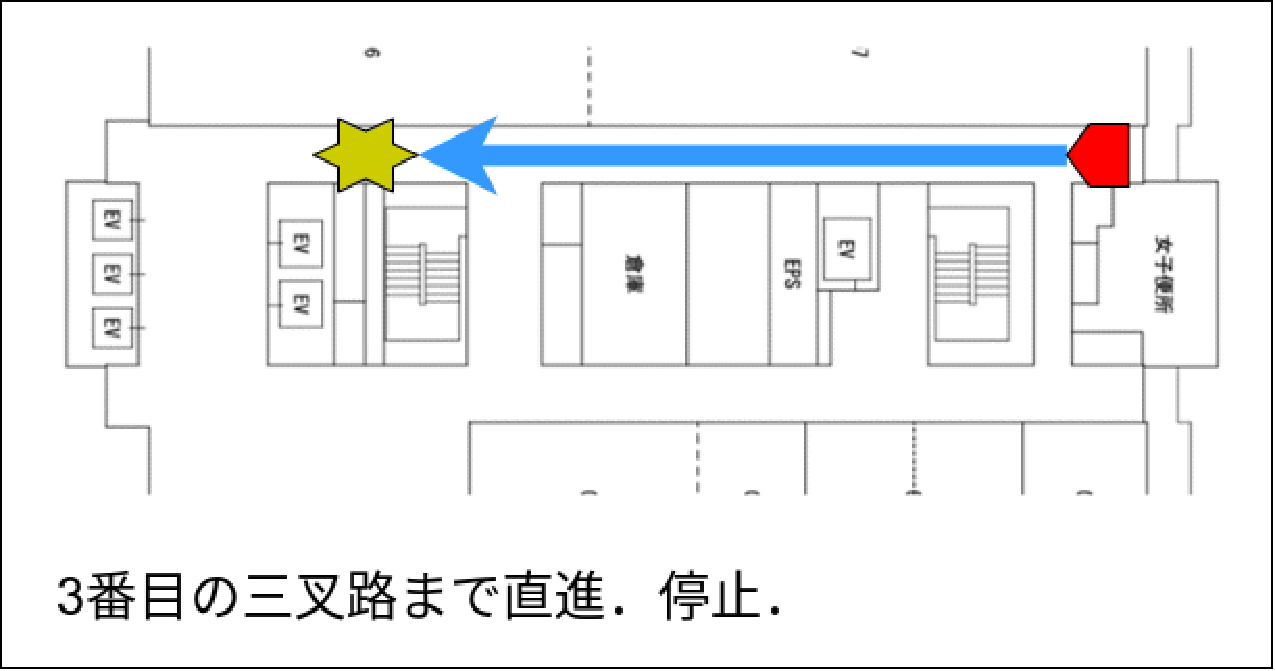
\includegraphics[keepaspectratio, width=57mm]{images/pdf/scenario/scenario01.pdf}
            \subcaption{Scenario 01}
            \label{composite}
        \end{minipage} &
        \begin{minipage}[t]{0.5\textwidth}
            \centering
            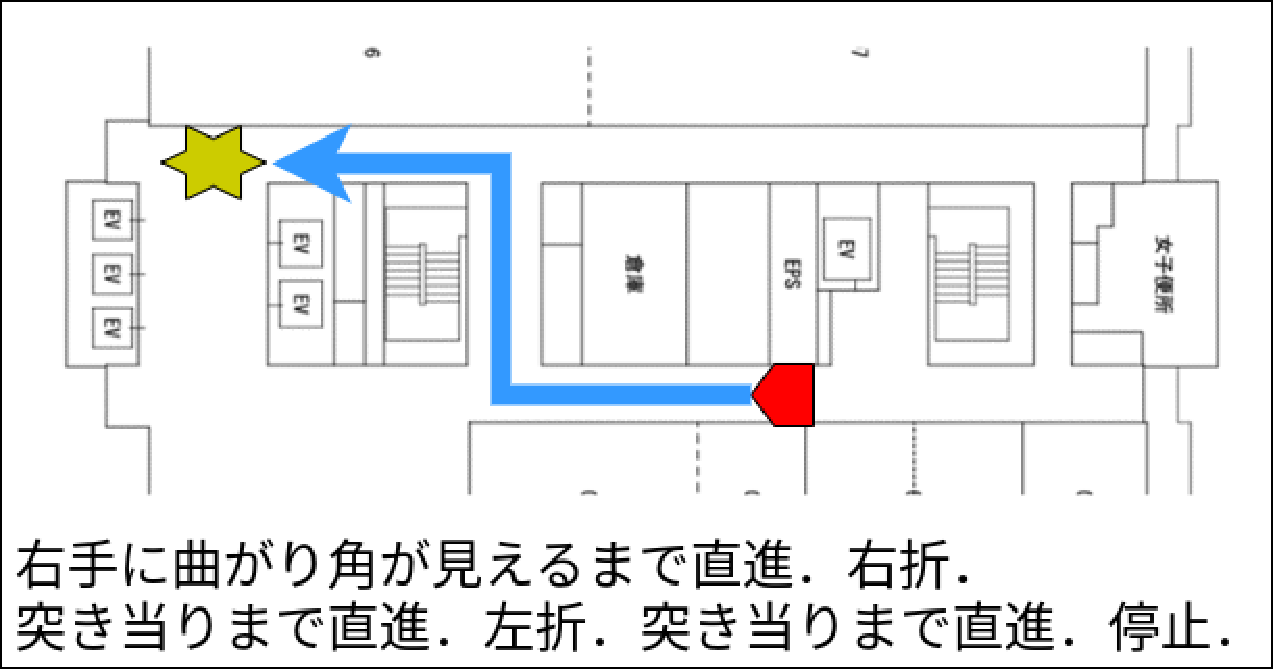
\includegraphics[keepaspectratio, width=57mm]{images/pdf/scenario/scenario02.pdf}
            \subcaption{Scenario 02}
            \label{Gradation}
        \end{minipage} \\
        \begin{minipage}[t]{0.5\textwidth}
            \centering
            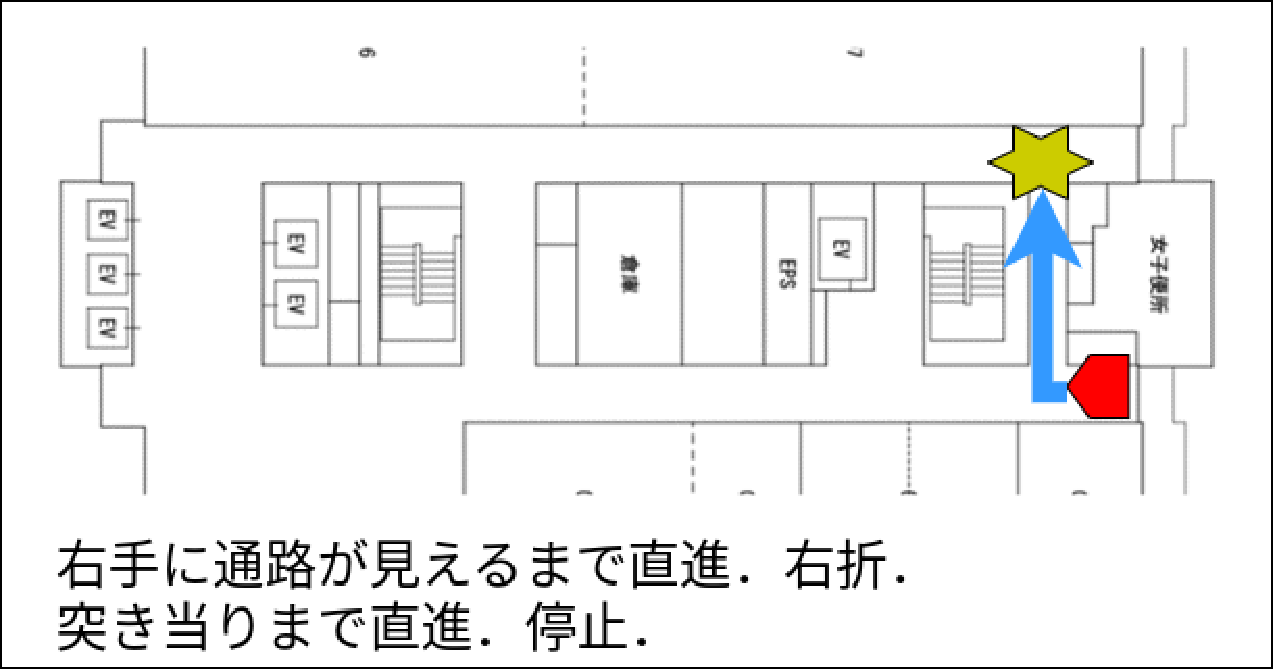
\includegraphics[keepaspectratio, width=57mm]{images/pdf/scenario/scenario03.pdf}
            \subcaption{Scenario 03}
            \label{fill}
        \end{minipage} &
        \begin{minipage}[t]{0.5\textwidth}
            \centering
            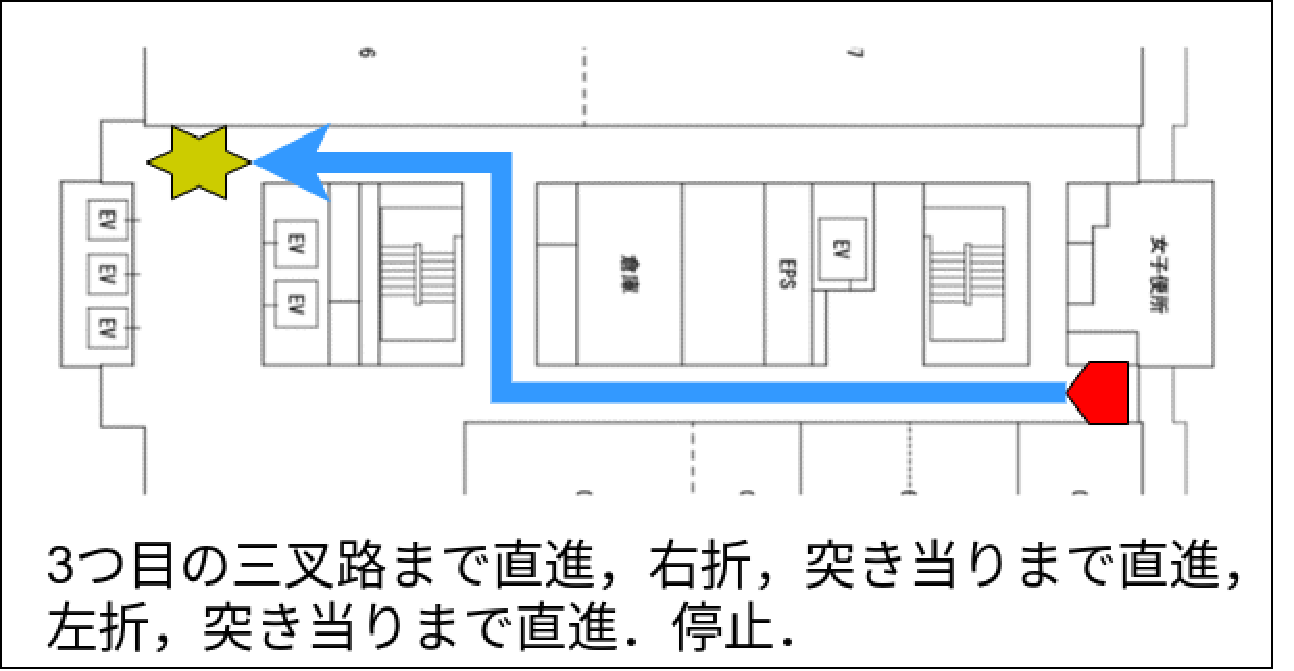
\includegraphics[keepaspectratio, width=57mm]{images/pdf/scenario/scenario04.pdf}
            \subcaption{Scenario 04}
            \label{transform}
        \end{minipage} \\
        \begin{minipage}[t]{0.5\textwidth}
            \centering
            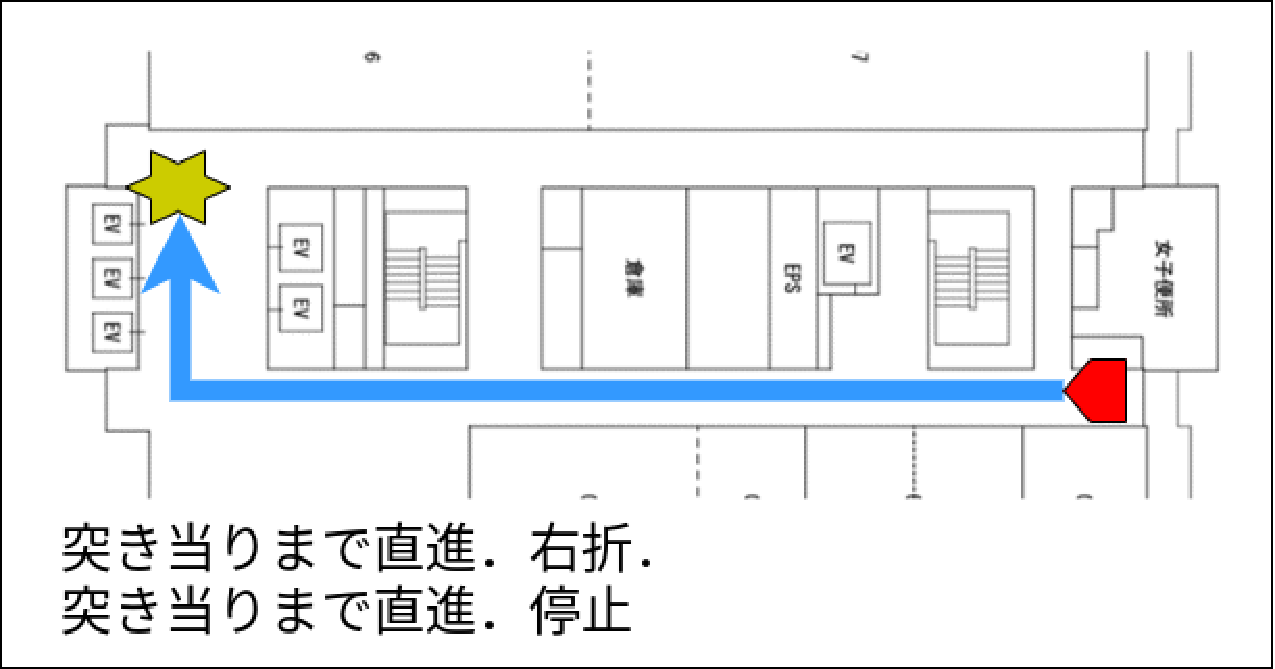
\includegraphics[keepaspectratio, width=57mm]{images/pdf/scenario/scenario05.pdf}
            \subcaption{Scenario 05}
            \label{image1}
        \end{minipage} &
        \begin{minipage}[t]{0.5\textwidth}
            \centering
            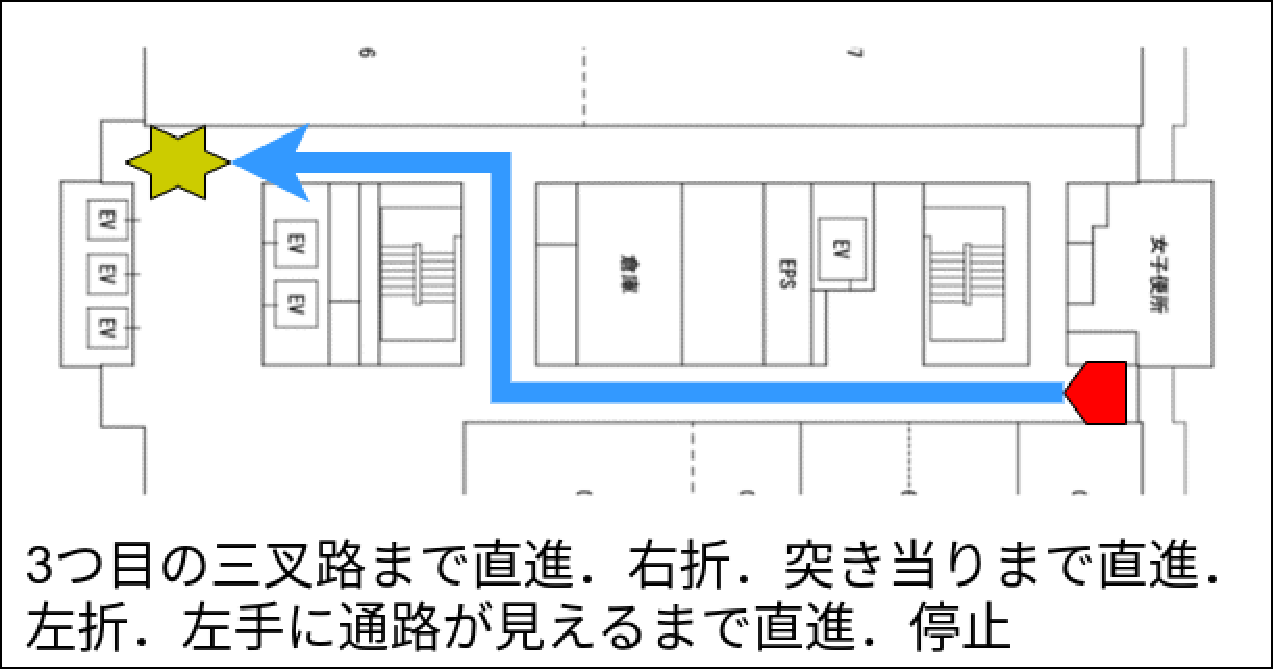
\includegraphics[keepaspectratio, width=57mm]{images/pdf/scenario/scenario06.pdf}
            \subcaption{Scenario 06}
            \label{fig:scenario24}
        \end{minipage}\\
        \begin{minipage}[t]{0.5\textwidth}
            \centering
            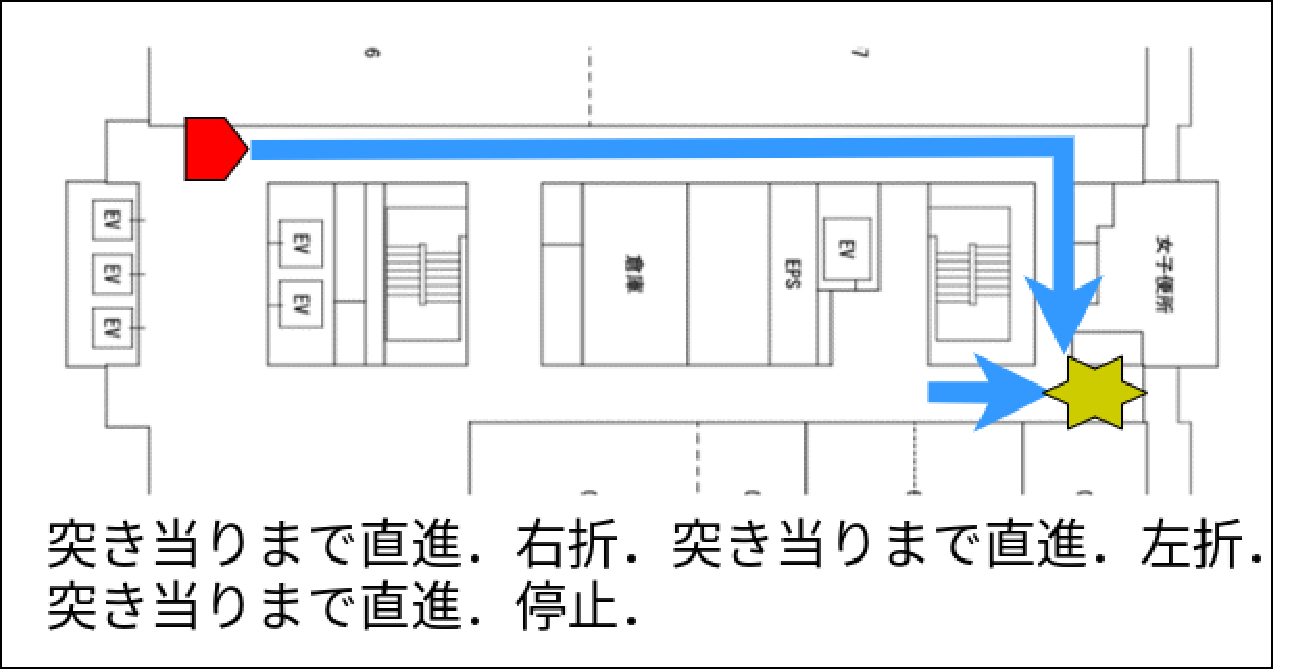
\includegraphics[keepaspectratio, width=57mm]{images/pdf/scenario/scenario07.pdf}
            \subcaption{Scenario 07}
            \label{imagess}
        \end{minipage}
    \end{tabular}
    \caption{Scenarios used in the experiment Quoted from \cite{haruyama2023}}\label{fig:scenario_exp}
\end{figure*}

\begin{figure}[htbp]
    \centering
     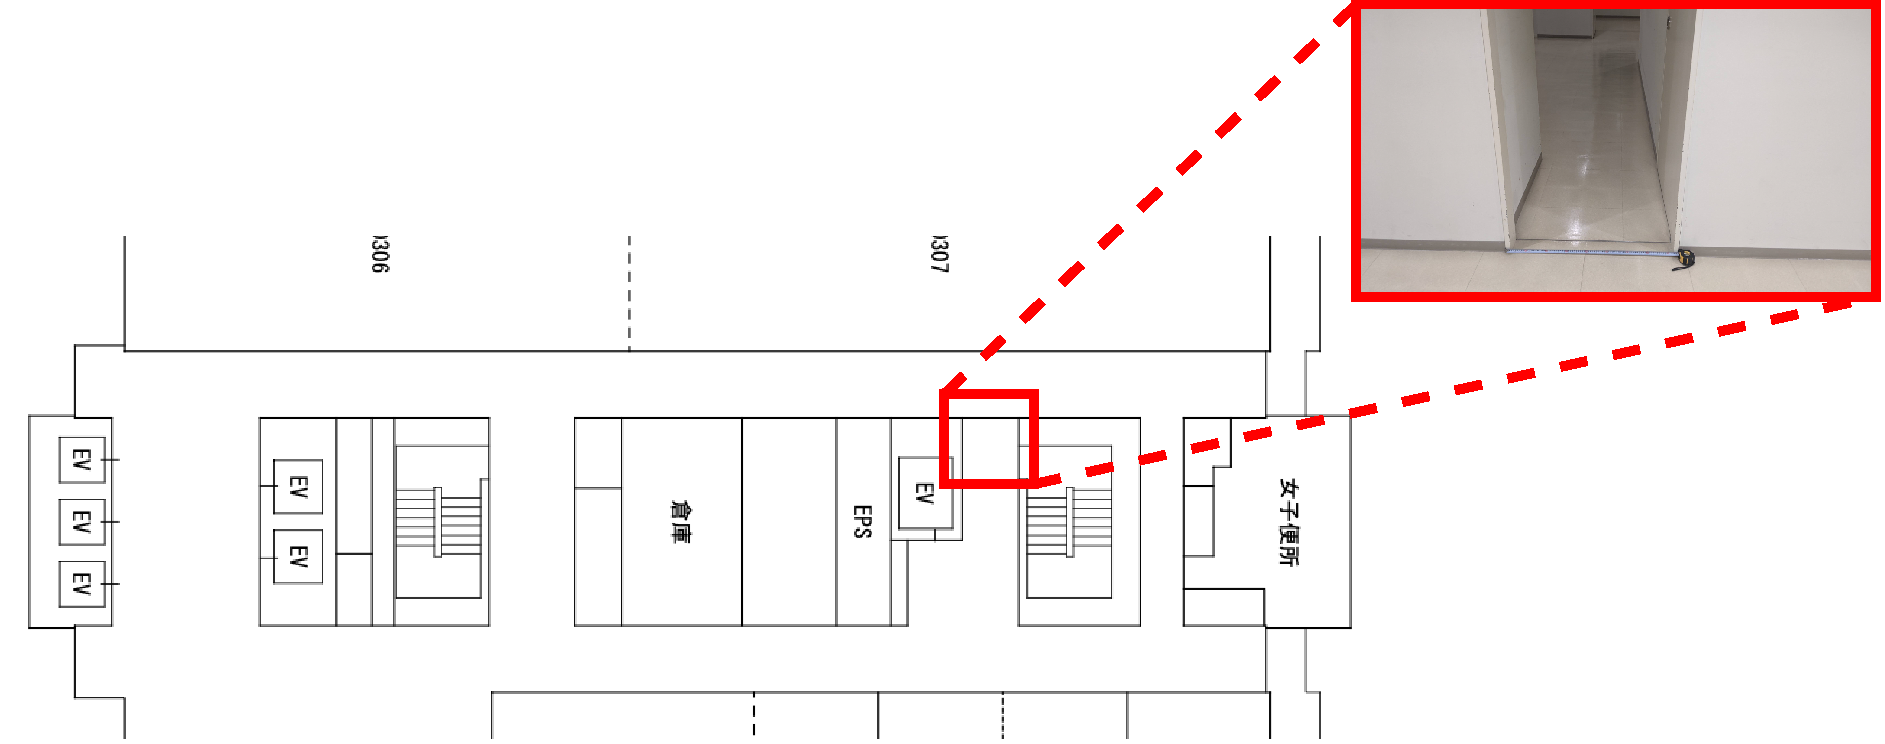
\includegraphics[width=100mm]{images/pdf/sce_semai.pdf}
     \caption{Experimental environment}\label{fig:semai}
\end{figure}

\newpage
\subsubsection{通路追従モジュールの訓練}
まずはじめに通路分類モジュールの訓練を行う.
前述の経路をメトリックマップに基づいたルールベース制御器の出力を用いて,
3周し,データセットを収集する.
収集したデータは,1,2 周目を訓練データとし,
3周目をテストデータとする.それぞれのデータ数は,
訓練データ 5781,テストデータ 2902 である. 
この訓練データ内のクラス間のデータ数は〜であり,訓練は
損失関数の重みを〜,バッチサイズを32として,30epoch行った.

訓練後,テストデータに対する通路分類モジュールの正解率{(Accuracy)},適合率{(Precision)}を計算する.
\begin{table}[htbp]
    \centering
    \caption{Number of classes in the dataset}\label{tab:target}
    \begin{tabular}{c|c|c}
    \hline
    Class & Learning data &Test data        \\
    \hline
    直進   & 2760 & 1377\\
    突き当たり   & 90 & 45 \\
    角(右) & 549 & 279 \\
    角(左)& 567 & 288 \\
    十字路 & 0 & 0 \\
    三叉路(右)& 753 & 387 \\
    三叉路(中央)& 306 & 153 \\
    三叉路(左) & 747 & 369 \\
    \hline
    \end{tabular}
\end{table}

\begin{table}[htbp]
    \centering
    \caption{cost}\label{tab:cost}
    \begin{tabular}{c|c}
    \hline
    Class & Class weights         \\
    \hline
    直進   & 1\\
    突き当たり   & 5\\
    角(右) & 5\\
    角(左)& 5 \\
    十字路 & 1  \\
    三叉路(右)& 5  \\
    三叉路(中央)& 10  \\
    三叉路(左) & 5  \\
    \hline
    \end{tabular}
\end{table}
\subsubsection{経路追従モジュールの訓練}
次に経路追従モジュールの訓練を行う.
通路分類モジュールの訓練と同様の経路を,
オンラインで 模倣学習しながら1周走行する.
その際のステップ数 は 12000 であった.

2つのモジュールを訓練後,シナリオを1例ずつ入力して,
ロボットの挙動を観察する.実験では,ロボットをシナリオの
スタート地点に移動して,自律移動を開始する.

\vspace{5zh}



\newpage
\subsection{実験結果}
テストデータに対する,通路分類モジュールの正解率と適合率を\ref{tab:result}に示す.
この計算にはpytorchのモデル評価用ライブラリである
torcheval\cite{torcheval}を用いて算出する.
\begin{table}[htbp]
    \centering
    \caption{Target direction and data for path-following module}
    \label{tab:result}
    \begin{tabular}{c|c}
    \hline
    指標 & 値        \\
    \hline
    Accuracy   & 0.98 \\
    Precision   & 0.4 \\
    \hline
    \end{tabular}
\end{table}
% \begin{table}[]
%     \centering
%     \caption{intersection あーだのコーダの}\label{tab:acc}
%     \begin{tabular}{|c|c|}
%     \hline
%     指標 & 値
%     \hline
%     accuraty & 0.98 \\
%     適合率 & 0.4 \\
%     \hline
%     \end{tabular}
% \end{table}
% \newpage

\ref{fig:exp_path}に\ref{fig:scenario_exp}のシナリオを入力した実験の様子を示す.
図に示すように入力されたシナリオの道順に従い, 三叉路などの分岐路
で適切に経路を選択して自律移動する様子が見られた.
結果として,7例すべてでロボットが, 目的地へ到達した.
以上の結果から, 提案するカメラ画像とシナリオに基づいて, 
経路を追従して目的地まで自律移動するシステムの有効性が確認された.

\begin{figure*}[htbp]
    \begin{tabular}{ccc}
        \begin{minipage}[t]{0.5\textwidth}
            \centering
            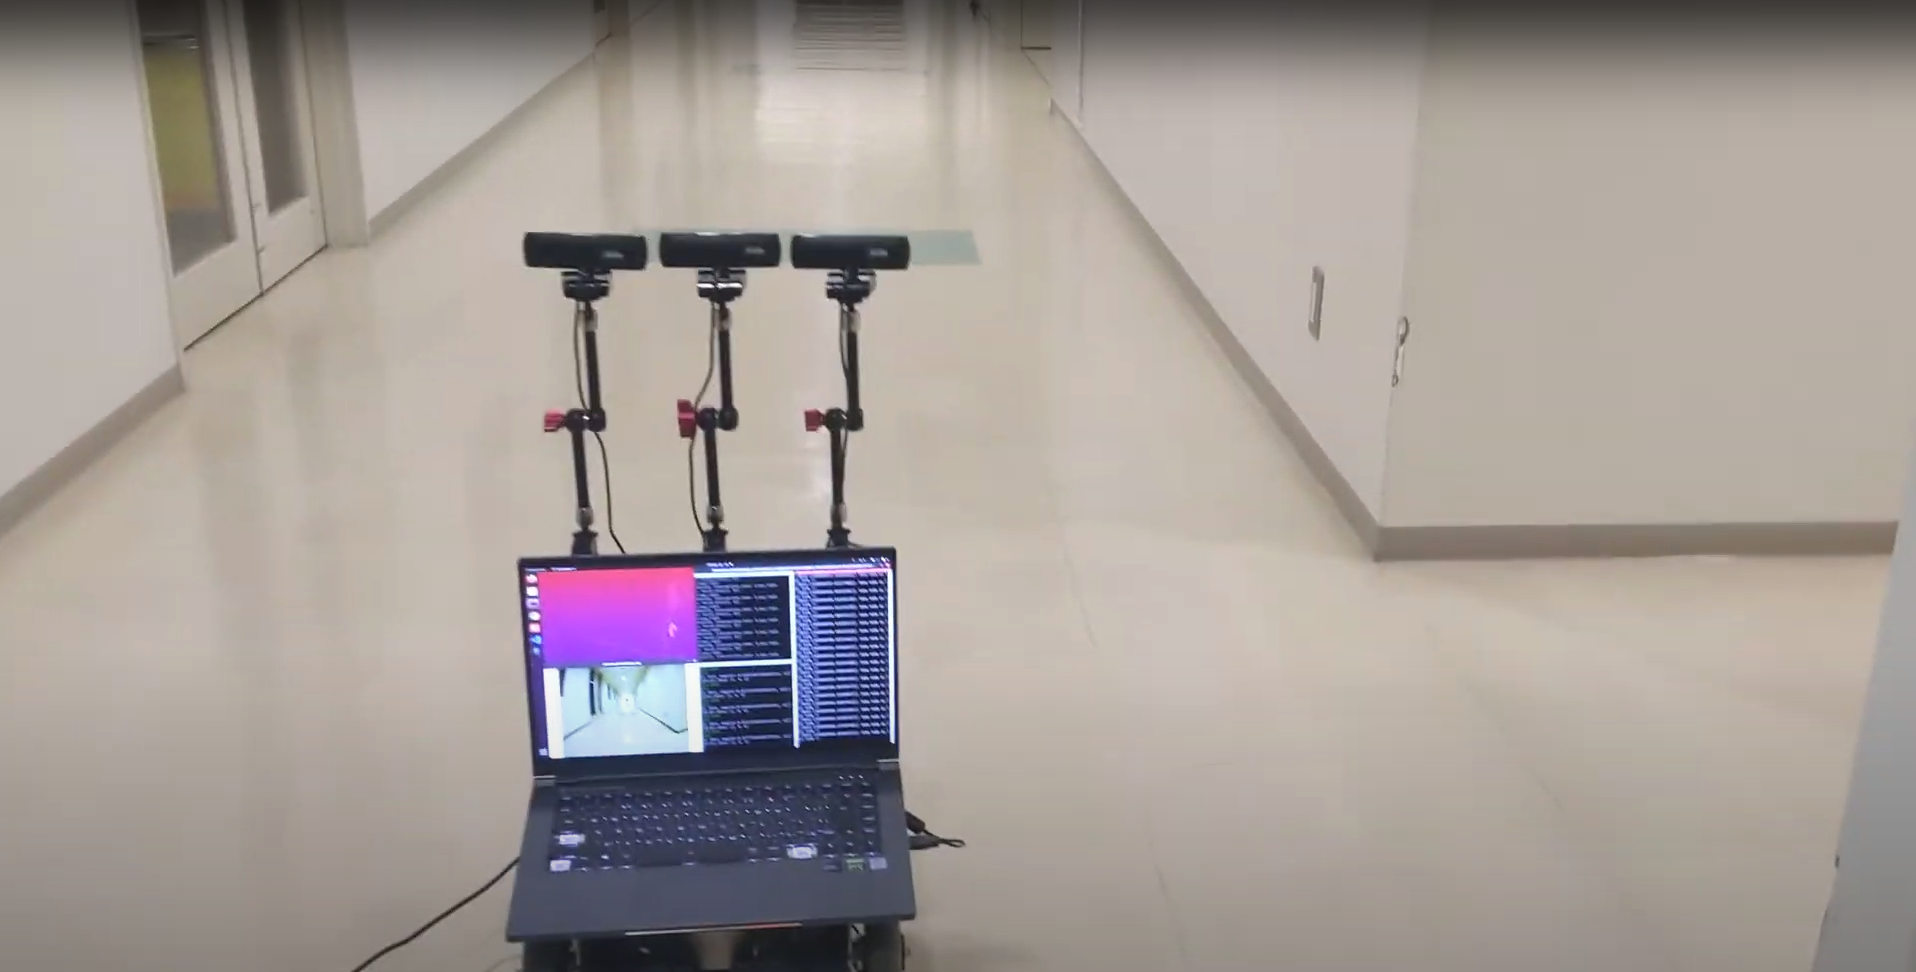
\includegraphics[keepaspectratio, width=70mm]{images/exp_path_follow_0.png}
            \subcaption{3つ目の三叉路まで直進(First 3-way)}
        \end{minipage} &
        \begin{minipage}[t]{0.5\textwidth}
            \centering
            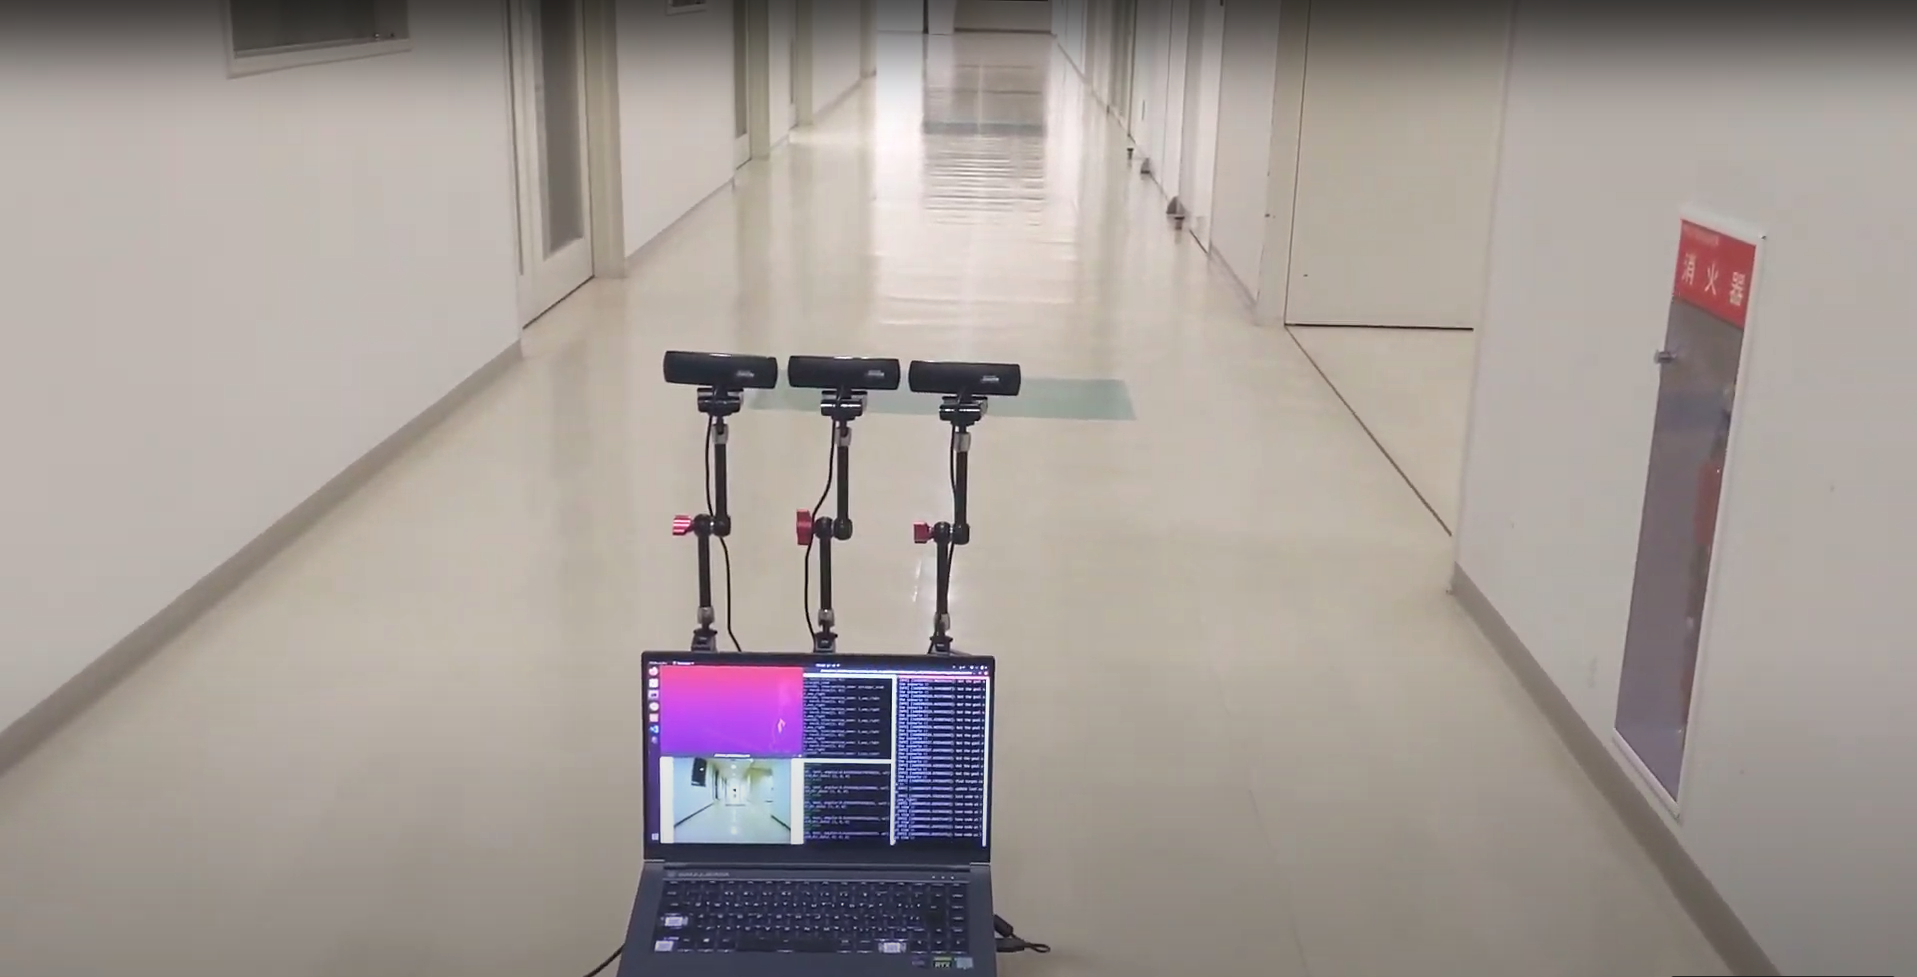
\includegraphics[keepaspectratio, width=70mm]{images/exp_path_follow_1.png}
            \subcaption{3つ目の三叉路まで直進(Second 3-way)}
        \end{minipage} \\

        \begin{minipage}[t]{0.5\textwidth}
            \centering
            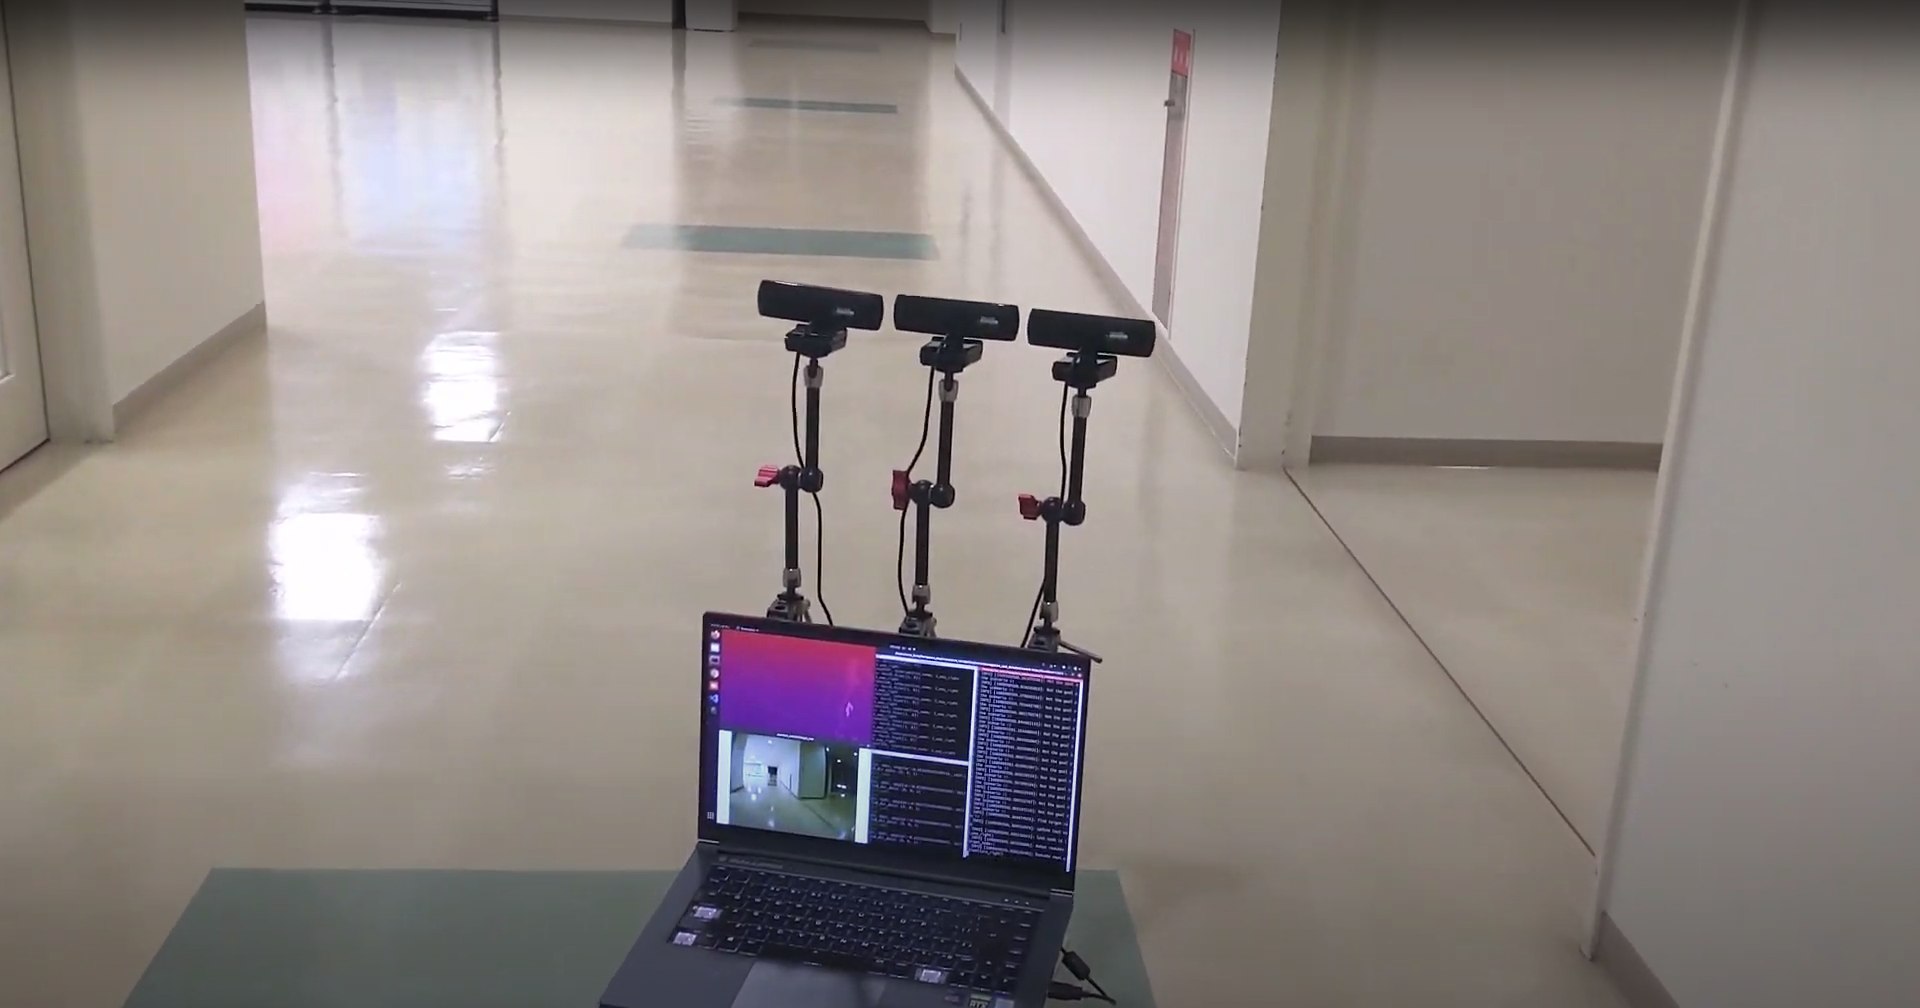
\includegraphics[keepaspectratio, width=70mm]{images/exp_path_follow_2.png}
            \subcaption{右折(Third 3-way)}
        \end{minipage} &
        \begin{minipage}[t]{0.5\textwidth}
            \centering
            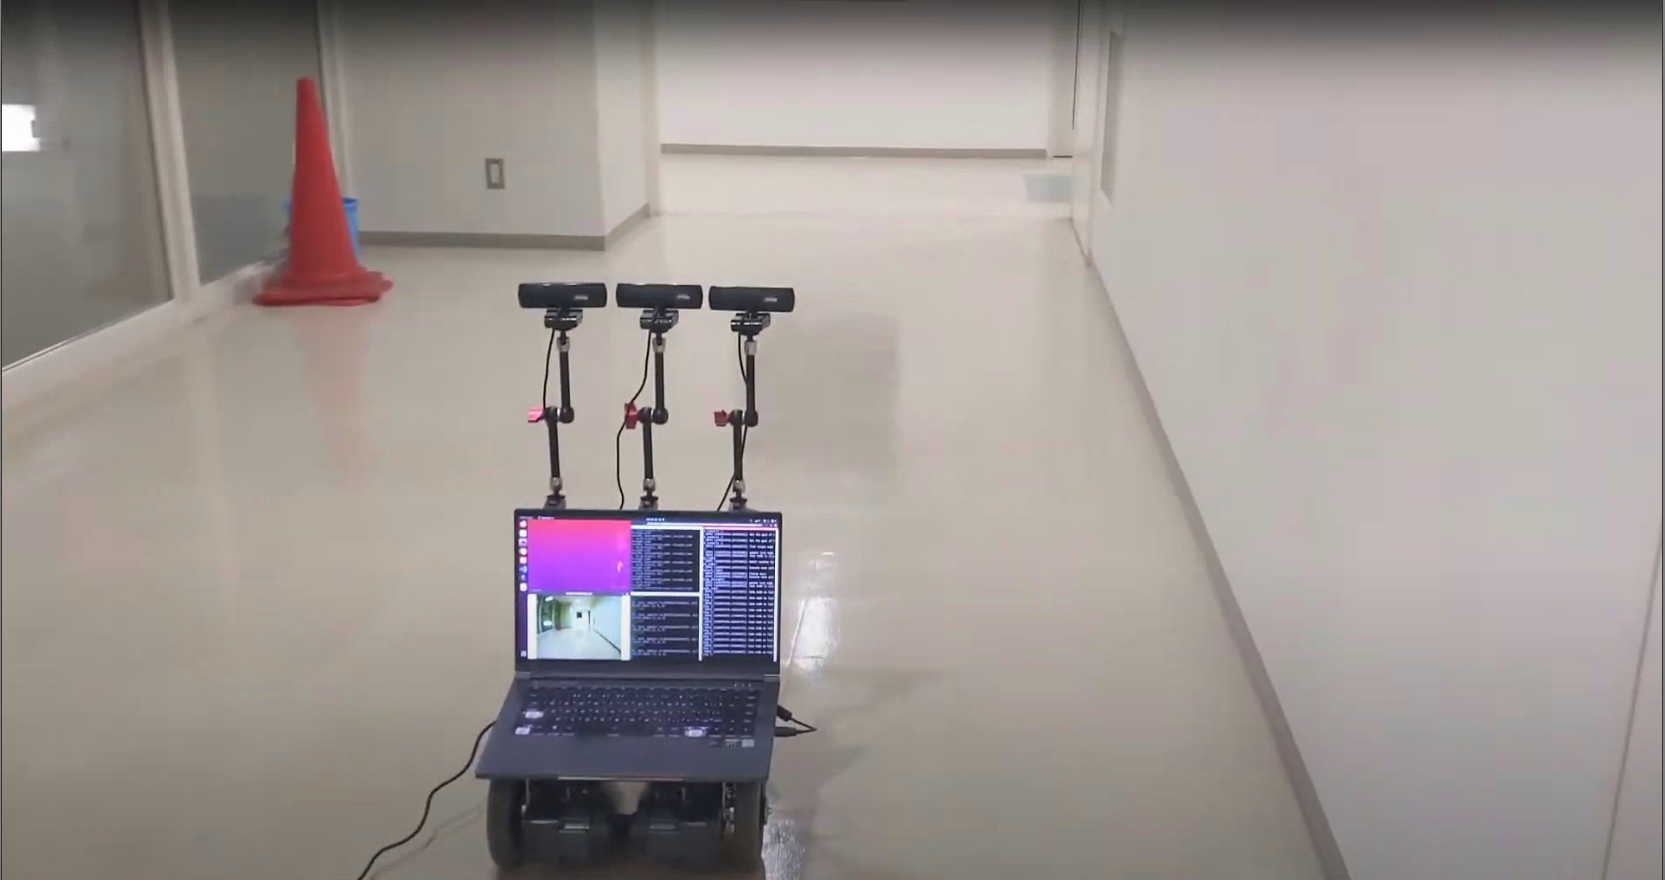
\includegraphics[keepaspectratio, width=70mm]{images/exp_path_follow_4.png}
            \subcaption{突き当たりまで直進(Straight road)}
        \end{minipage} \\
        \begin{minipage}[t]{0.5\textwidth}
            \centering
            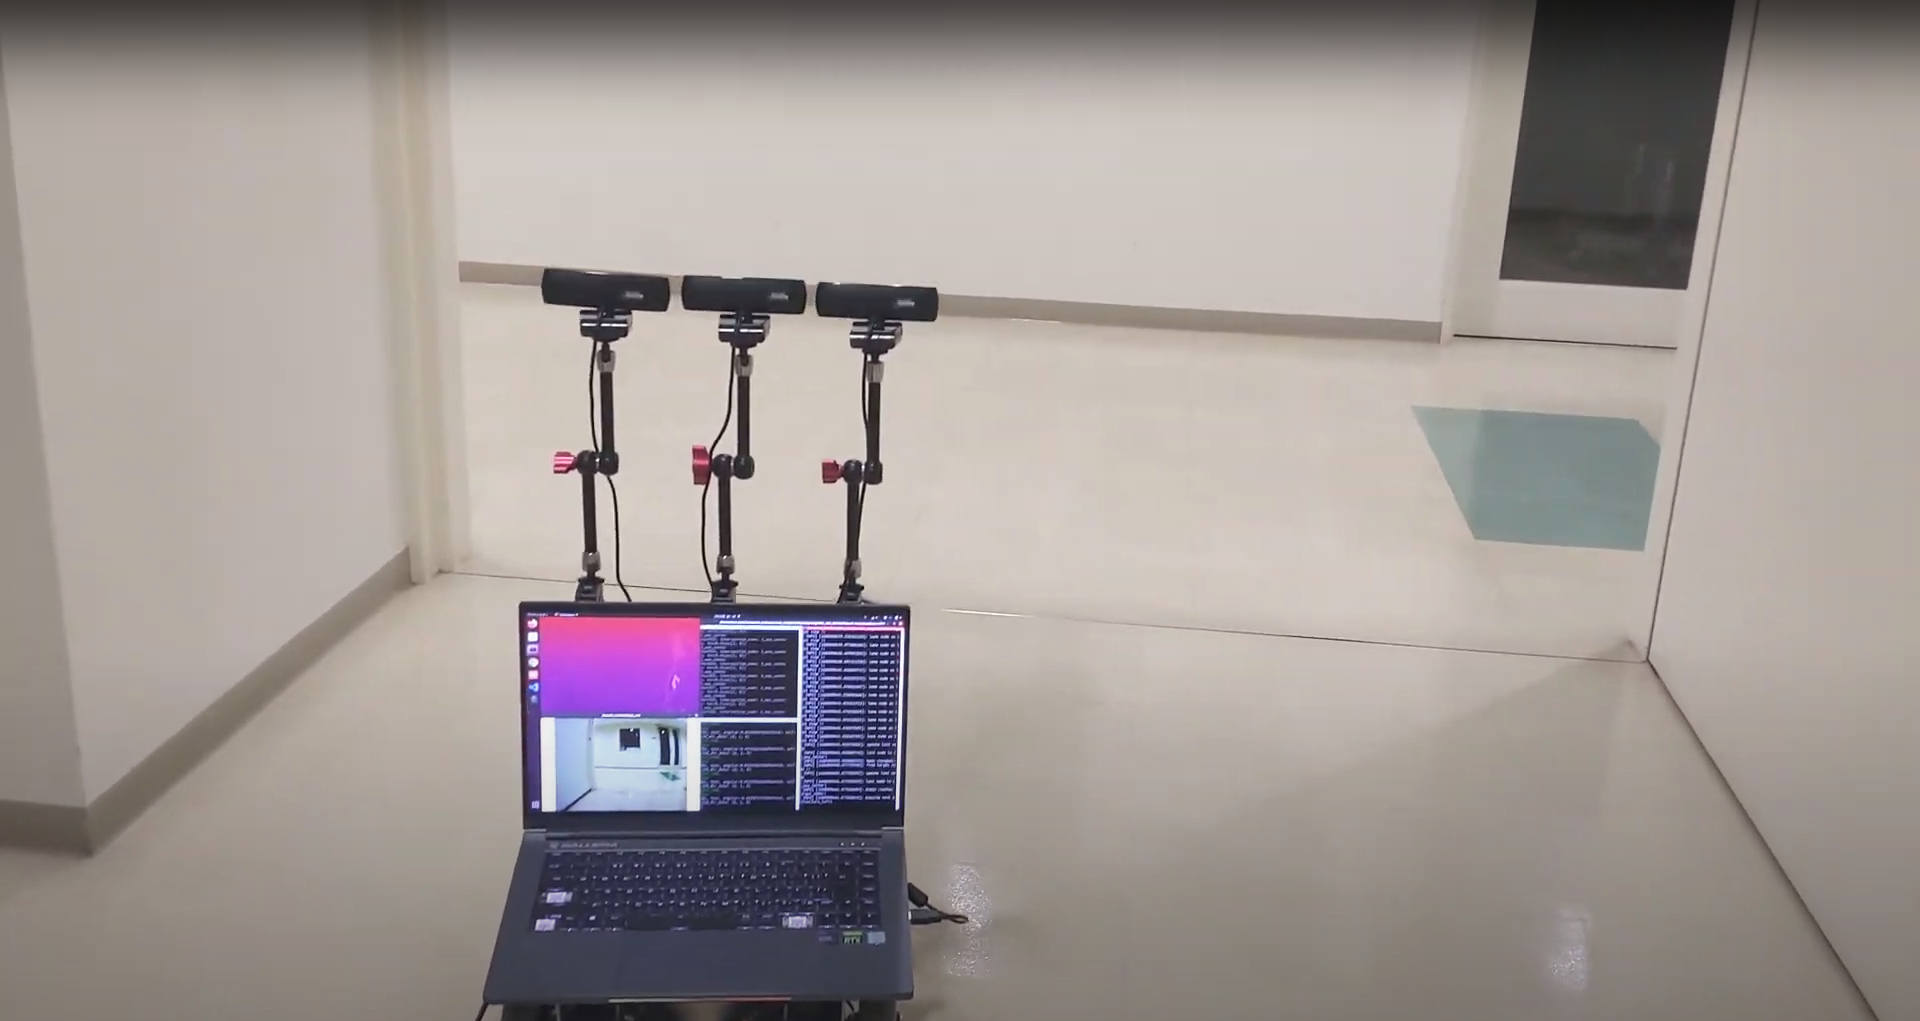
\includegraphics[keepaspectratio, width=70mm]{images/exp_path_follow_5.png}
            \subcaption{左折(End)}
        \end{minipage} &
        \begin{minipage}[t]{0.5\textwidth}
            \centering
            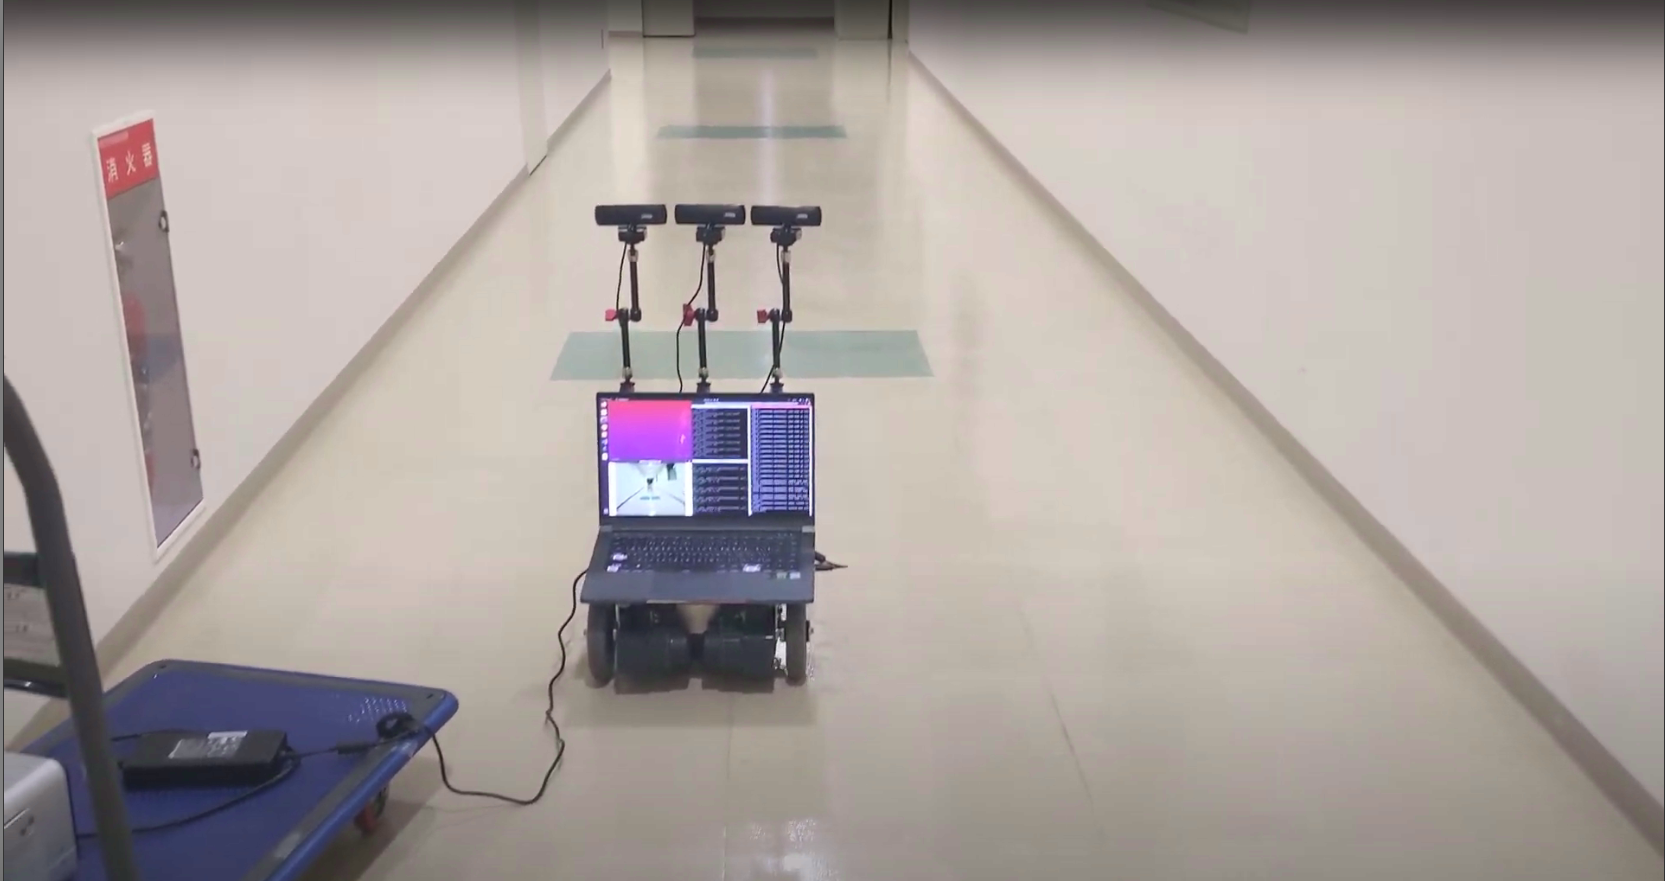
\includegraphics[keepaspectratio, width=70mm]{images/exp_path_follow_6.png}
            \subcaption{突き当たりまで直進(Straight road)}
        \end{minipage} \\
        \begin{minipage}[t]{0.5\textwidth}
            \centering
            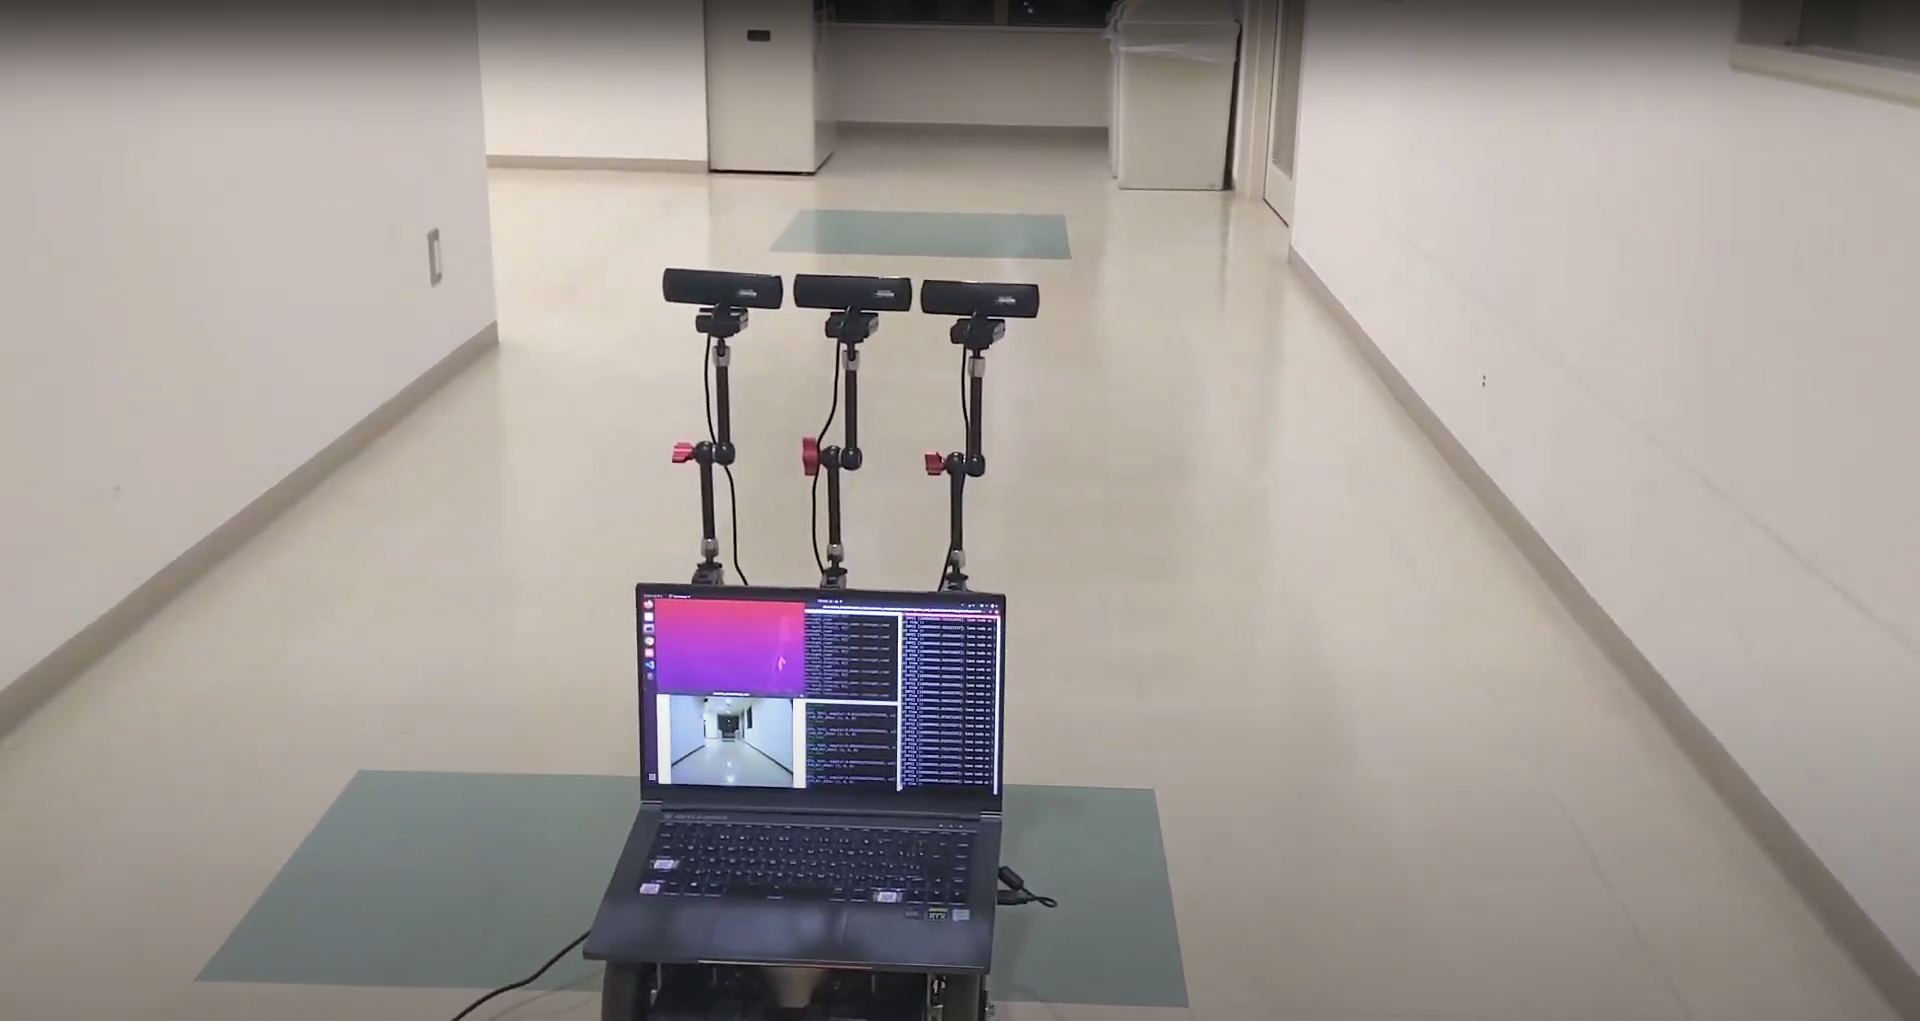
\includegraphics[keepaspectratio, width=70mm]{images/exp_path_follow_7.png}
            \subcaption{停止(End)}
        \end{minipage}
    \end{tabular}

    \caption{An example of the robot applied the proposed system Quoted from \cite{haruyama2023}}\label{fig:exp_path}
\end{figure*}